\documentclass[conference]{IEEEtran}
\IEEEoverridecommandlockouts
% The preceding line is only needed to identify funding in the first footnote. If that is unneeded, please comment it out.
\usepackage{cite}
\usepackage{amsmath,amssymb,amsfonts}
\usepackage{algorithmic}
\usepackage{graphicx}
\usepackage{textcomp}
\usepackage{xcolor}
\usepackage{caption}
\usepackage{subcaption}
\usepackage{url}
\usepackage{outlines}
\usepackage{hyperref}
\usepackage{float}
\usepackage{enumitem}
\usepackage{mathtools}
\usepackage{tikz}
\usetikzlibrary{arrows.meta,positioning}
\def\BibTeX{{\rm B\kern-.05em{\sc i\kern-.025em b}\kern-.08em
    T\kern-.1667em\lower.7ex\hbox{E}\kern-.125emX}}
\newcommand{\photo}[1]{%
\includegraphics[width=8cm, height=5cm]{#1}
}

\begin{document}

\title{Utilizing Reinforcement Learning with Path Planning Algorithms to Create More Efficient Paths of Travel\\
}

\author{\IEEEauthorblockN{Andrew Meyer}
\IEEEauthorblockA{\textit{Robotics Engineering } \\
\textit{Worcester Polytechnic Institute}\\
Worcester, Massachusetts \\
ameyer2@wpi.edu}
\and
\IEEEauthorblockN{Everett Wenzlaff}
\IEEEauthorblockA{\textit{Robotics Engineering } \\
\textit{Worcester Polytechnic Institute}\\
Worcester, Massachusetts \\
ecwenzlaff@wpi.edu}
\and
\IEEEauthorblockN{Sushant Raj}
\IEEEauthorblockA{\textit{Robotics Engineering } \\
\textit{Worcester Polytechnic Institute}\\
Worcester, Massachusetts \\
skraj@wpi.edu}}

\maketitle

\begin{abstract}
In this report, the implementation of a reinforcement learning algorithm in conjunction with multiple basic path planning algorithms is investigated
to determine if reinforcement learning can efficiently optimize a simulated TurtleBot in a 2D environment based on the manipulation of several key
parameters with the performance measured against path length, smoothness, travel time, velocity, and clearance. The simulations under study were
conducted with ROS2 in a Gymnasium environment using open-source Turtlebot code and a Nav2 stack. The reinforcement learning algorithm was designed to
utilize MPPI and DWB path planners and as a result, optimize them to perform better than their current offline counterparts.
\end{abstract}

% Required sections: Introduction (Importance, objectives, related work), Materials & methods (Simulation setup: Turtlebot, ROS2, Code building
% process, RL & reward function), Experiments (MPPI and/or DWB w/ and w/o RL), Results (same as experiment), Discussion (Implications, future work)

\section{Introduction}
    \subsection{Current state of the Art}
    In the industrial environment of Autonomous Mobile Robots (AMRs), path planners are generally deployed en-masse and are not tailored to the
    customers or environment needs in which they are deployed. This results in good, but not excellent, performance and, while easier to maintain on
    the backend, can limit customer output on the front end. These general deployments often cast a wide net and aim to operate on the ``safe side'',
    whether that be wide, nonadjustable clearance, paths around high traffic areas, or creating lanes that avoid foot traffic altogether. In reality,
    each customer has different needs and, outside of required safety standards, may have certain workplace standards that could offer better
    performance if utilized properly to tune the AMR deployment. It is obvious that hand tuning any number of parameters for each individual
    deployment site is unreasonable and the time spent on it would far outweigh any long-term benefits. Additionally, the deployment time for
    standard AMRs can be several weeks, meaning there is a potential for downtime when looking at brownfield sites. Implementing a reinforcement
    learning (RL) algorithm paired with machine vision such as LiDAR could reduce that deployment time from weeks to days, as all the training is
    done on the back end and there is no need to manually set path layouts.
    
    \subsection{Project Objectives}
    To reduce the amount of manual input needed to tune path planner parameters, a reinforcement learning (RL) algorithm is deployed into the simulation for a period of
    raining and the following parameters are adjusted to optimize the Turtlebot travel across the simulated warehouse: Clearance, Accuracy,
    Efficiency, and Smoothness. These four parameters have been previously proven to be statistically significant modifiers for both path planners 
    under study \cite{b1} \cite{b2}. In this context, a dense reward function is custom-built to help direct the RL algorithm through each episode so
    that when it is deployed, it can be more lightweight in terms of computational load.

    \subsection{Background}
    While modern RL algorithms are a fairly new technology, AMRs and their predecessors, Automated Guided Vehicles (AGVs), are not and have been in
    use for over 70 years in various forms. Similarly, path planners such as Model Predictive Path Integral (MPPI) and Dynamic Window Approach-Based
    (DWB) are 10-15 years old. As a result, there is a wide breadth of research into existing literature that has been conducted to both verify plausibility as well as serve
    as a reasonable set of starting points.
        
        \subsection{Path planning}
        Elbouhy et. al designed a study that consisted of three different path planners that were tested in environments with static and dynamic
        obstacles and the results were then evaluated to compare algorithms. The study analyzed DWB, MPPI, and RPP (Improved Pure Pursuit) planners
        and used the following criteria to determine path quality: time, distance, smoothness, minimum clearance, runs completed, and number of
        recoveries. This study showed that MPPI was the fastest but least smooth, DWB operated with the least clearance, and RPP took the most time
        and traveled the longest distance \cite{b1}. This demonstrates that different planners have different strengths and weaknesses which
        ultimately led to the initial integration of both MPPI and DWB into the RL-based simulation built in this project.
        
        Li et. al studied the Dynamic Window Approach (DWA) algorithm and adjusted evaluation parameters in an effort to optimize the path planning.
        The evaluation function utilized in this paper looked at the heading, the distance between the trajectory and nearest obstacle, and the speed
        of the robot, along with weighted modifiers of each. A simple environment was setup and the tuning modifiers were adjusted for optimization
        \cite{b2}. In the context of this project, the interest lies in the tuning equation itself; and Li's tuning equation provided a 
        confident proof-of-concept that path planning algorithms can be tuned and optimized on a limited number of parameters and the results are
        statistically significant and positive.

        \subsection{Reinforcement Learning}
        Qu et. al. presented a method of training an RL policy offline to accelerate the convergence for the online control of MPPI in an unmanned
        aerial vehicle (UAV). The method they proposed involved utilizing the Distributional Soft Actor-Critic (DSAC) algorithm to have an RL agent
        train a pair of neural networks to model distributions for the control costs and roll-out guiding policy used directly within the online MPPI
        control. This improved MPPI by providing better ``first guesses'' than standard MPPI. The results of their experiments showed that their
        method converged significantly faster, produced smoother trajectories, and provided higher success rate in reaching the goal than standard
        MPPI \cite{b3}. The guiding principle of this paper translates directly to this project to enhance the strengths of existing local planners
        instead of replacing them by leveraging the strengths of both RL and traditional path planning algorithms to create a more efficient and 
        adaptable path planning solution for mobile robots in complex environments.

        Ting et. al. presented a modified Proximal Policy Optimization (PPO) in conjunction with a deep reinforcement learning (DRL) algorithm in
        order to reduce the time needed to move an agent through an environment. To reduce the number of episodes required and thus the calculation
        time for each move, they proposed a distance-based weighted dense reward function. The reward function they proposed utilized the euclidean
        distance to the goal to provide a higher value reward for better steps \cite{b4}. Since this reward function is not strictly linked to PPO
        parameters, the concept can easily translate into both MPPI and DWB that are utilized for the training in this project. 

        Debnath et al. propose a modular navigation framework for navigation that combines a classical global planner with a DRL based local planner.
        The global planner generates waypoints and assigns Gaussian soft costs around detected pedestrians to anticipate their future positions,
        while the trained local planner dynamically follows these waypoints while avoiding imminent collisions in real time. The reward function used
        to train the local planner includes eight terms covering goal reaching, collision penalties, waypoint tracking progress, pedestrian proximity
        avoidance, and a small per-timestep penalty to encourage efficiency. Through experiments, their hybrid system outperformed both a traditional
        DWA planner and a standalone RL baseline, with the RL-augmented system achieving a notably lower collision rate \cite{b9}. This paper is
        directly relevant to the dynamic parameter tuning approach adopted in this project where the RL agent observes local state and adjusts planner
        parameters throughout the navigation process rather than making a single configuration decision upfront.

        Rana and Kaveendran implemented a PPO-based DRL agent to train a TurtleBot3 navigation policy from scratch within a ROS2 environment. The
        agent observes the robot's surroundings through a LiDAR scan and directly outputs normalized linear and angular velocity commands at each
        timestep, making it the sole navigation controller rather than an augmentation of an existing planner. Training was conducted using a
        two-term reward function including a small positive reward for forward progress and a large negative penalty for collisions. The trained
        policy resulted in better performance, and behavior improvements such as slowing near tight spaces \cite{b10}. This paper is particularly
        relevant as a validation of a similar implementation being used in this project: ROS2, Gymnasium, PPO, and a TurtleBot platform. The key
        distinction is that their RL agent replaces the planner entirely by outputting direct velocity commands, whereas this project's agent acts as
        a meta-controller. Their training time was approximately four hours for a significantly harder problem (the agent must learn full navigation
        from raw sensor data), providing reassurance that the team's proposed approach is viable.

        \subsection{Other Noteworthy Resources}
        In addition to the papers described in detail above, there were several other papers that were reviewed which provided supplemental
        information for shaping the project. \cite{b5} and \cite{b6} provided metrics and insights on planner path evaluation which was utilized as
        inspiration for the evaluation metrics implemented in this project. \cite{b7} and \cite{b8} demonstrated more examples which utilized RL
        within some sort of path planning framework for a mobile robot (including both direct and indirect RL control), again reinforcing the
        possibility of the concept explored in this project.
        
        While there are several papers which demonstrate the use of RL in path planning, no papers were identified which explicitly utilized RL to
        configure the parameters for a given local path planning algorithm. This is a critical gap in the literature and study of this field, as it
        is well established that the performance of local path planners can be highly sensitive to their parameter settings, and that optimal settings
        can vary significantly across different environments and use cases. Meanwhile, some of the examples utilizing direct RL control are not very
        extensible as these methods tend to only train the RL agent to operate in a specific environment; and re-training for more complex
        environments can be very costly. By leveraging RL to automatically tune these parameters, this project theoretically fills this gap and
        demonstrates a novel approach to optimizing path planning performance in a way that is adaptable to the specific needs of different
        deployment sites.

\section{Materials and Methods}\label{sec:pq_metrics}
    \subsection{Simulation Setup}
    In order to reduce the scope and complexity of the required programming of this project, an RL agent was implemented within ROS2. Using ROS2
    prevents needing to develop a simulation environment and navigation stack from scratch; which allows for more dedicated effort to developing
    the RL infrastructure and evaluating performance. Additionally, the simulation environment is constrained to a 2D grid with a TurtleBot robot
    model in order to simplify the state space and holonomic constraints for the path planners and RL infrastructure, again to avoid adding unnecessary complexity.
    
    The environment was designed to be cross-platform and reproducible, leveraging Docker to encapsulate all dependencies and ensure
    consistent behavior across the team's Mac, Windows, and Linux development machines. The environment is structured as a two-layer Docker image:
    a base capstone\_ros\_layer image that installs all system-level dependencies (ROS2, Nav2, TurtleBot4 description packages, and visualization
    tools), and a top-level rbe\_capstone image that layers in the project's ROS2 workspace. Separating dependency installation from application
    code allows the more expensive base layer to be rebuilt infrequently while code iteration remains fast.

    The simulation runs on ROS2 Jazzy with the CycloneDDS middleware layer for inter-node communication. The robot model used is the TurtleBot4,
    whose URDF is loaded via \texttt{xacro} and published to the \texttt{/robot\_description} topic by the \texttt{robot\_state\_publisher} node.
    Navigation is performed in a 2D occupancy grid environment using the Nav2 stack, which includes \texttt{nav2\_map\_server} for loading pre-built
    maps and \texttt{nav2\_lifecycle\_manager} for managing the life cycle of navigation nodes. Maps are stored as paired \texttt{.pgm} and
    \texttt{.yaml} files and are selectable at launch time, enabling the team to quickly swap between different warehouse environments as the project
    progresses.

    Visualization is handled by RViz2, which renders the robot model, occupancy map, and planned paths. For the purpose of this project, RViz2 is chosen
    over Gazebo for visualization because it is more lightweight and the scope of this project does not require a full physics simulation. Gazebo will
    be consistently slower in launching and running episodes, which is not ideal for iterative tests and tuning of the RL algorithm. RViz2 provides
    sufficient visualization capabilities for the 2D occupancy grid and planned paths while allowing for faster iteration cycles. To further speed up iterative
    development, launch files are configured to bring up all required nodes: the robot state publisher, static TF broadcasters, map server, life cycle manager,
    and RViz2, making it straightforward to launch the full environment with a single command. 

    \subsection{Performance Evaluation Criteria}
    % Moving this back here to introduce the criteria as a sort of "guiding tenet" for our "reward function framework" introduced in the RL Architecture section below
    In order to assess the impacts of incorporating RL within the local path planning process, relevant path quality metrics were identified throughout our literature review for evaluating path planner performance. These path quality metrics can be summarized by the following criteria:
    \begin{itemize}
        \item Safety (clearance from obstacles)
        \item Accuracy (success rate in reaching the goal, amount of deviation from global path plan, etc.)
        \item Efficiency (total time and distance to goal)
        \item Smoothness (heading angle variance, velocity variance, etc.)
    \end{itemize}

    The path quality criteria listed above ultimately served as the foundation for the performance evaluation of the RL-augmented planner against the baseline planner with standard parameters. Additionally, since it was decided that these criteria would be tied directly to performance; these criteria were also worked directly into our reward function design in order to shape training for the RL agent.

    \subsection{RL Architecture}
    The RL component of the project is a trainable agent that tunes planner parameters directly through the Nav2 stack. Independent from the
    specific path planning algorithm and RL learning algorithm, two design options were initially explored for overall architecture of the states and actions: a one-time parameter tune, or a
    dynamic parameter tuning. It was decided that the implementation and expected results of a dynamic RL application would be favorable and feasible
    within the scope of this project. With this approach, the RL agent would be responsible for dynamically tuning the local planner's parameters throughout
    the navigation process; where the agent's state (observation) vector at each time step includes information about what the robot can perceive (e.g. current pose, velocity, distance from the goal, obstacle cost
    of the surrounding environment, etc.), and the agent's action vector is responsible for adjusting the planner parameters (via a continuous action space) at each timestep. To support frequent
    observations and actions throughout the navigation process, the reward function is designed to encourage efficient, smooth, and safe navigation by providing
    positive rewards for progress towards the goal and negative rewards for collisions, long travel times, and time spent in close proximity to obstacles. The
    goal of these rewards is to encourage the agent to learn how to guide the robot through crowded environments as smoothly and quickly as possible.

        \subsubsection{Training Framework}
        Training is driven by the Stable-Baselines3 (SB3) library, which interfaces with the simulation through a custom Gymnasium environment.
        SB3 is widely used for training RL agents and provides a variety of algorithms and utilities for training and evaluation, but one challenge that we had to
        consider is that it is designed for synchronous environments. This project heavily relies on ROS2, which is fundamentally an asynchronous setup with multiple
        nodes communicating through topics and services. The main training loop needs to block and wait for new observations and rewards from the ROS2 environment, but
        also needs to be able to control the asynchronous ROS2 nodes and services to set up and run each episode. To bridge this gap, a state machine-like architecture
        was implemented to allow the main training loop to operate synchronously with each episode. This was achieved by setting up a thread queue to put the main
        training loop in charge of the episode flow, where the loop listens to the metrics from a ROS2 topic, and then issues service calls to control the episode flow
        (start episode, switch planners, update parameters) based on those metrics.
        
        To evaluate which reinforcement learning strategy would be most effective for dynamically tuning planner parameters and maximizing the reward function, two RL design approaches were explored in parallel using two different RL algorithms: PPO and Soft Actor-Critic (SAC). Each offers distinct advantages in continuous‑control settings, and comparing them directly allows analysis of their computational costs, sample efficiency, and stability characteristics within the constraints of a ROS2‑based navigation environment. By training both agents on the same environment, a determination could be made on whether one algorithm demonstrated more favorable results in a simple 2D navigation environment.  
        
        PPO is an on‑policy actor-critic RL algorithm that updates its policy using batches of freshly collected trajectories (rollouts). Its defining feature is a clipped objective that restricts how far the policy is allowed to move during each update, which helps maintain stability during training. PPO is widely used because it strikes a balance between implementation simplicity, robustness, and reliable convergence across many continuous‑control tasks. Conceptually, PPO learns by repeatedly sampling new experience, computing policy gradients from that experience, and applying carefully constrained updates that prevent the policy from changing too abruptly.
        
        SAC is an off‑policy actor–critic RL algorithm that learns from a replay buffer of past transitions rather than relying solely on newly collected data. SAC optimizes expected return and policy entropy, encouraging the agent to maintain broad exploration throughout training. This entropy‑regularized objective makes SAC highly sample‑efficient and well suited for environments where each interaction step is expensive to generate. At a high level, SAC continuously improves both a stochastic policy and a pair of Q‑value critics using stored experience, enabling stable learning even in high‑dimensional continuous action spaces.

        While the specific reward functions ultimately deviated between the two different RL design approaches, the overall design of the reward functions were the same. The overall design involved a hybrid reward function which included terms for both dense and sparse rewards based on the relevant path quality evaluation criteria. The dense rewards for both approaches (calculated on a per time step basis) were shaped by progress made toward the goal (Efficiency), commanded angular velocities (Smoothness), and proximity to obstacles (Safety). The sparse rewards for both approaches involved issuing large positive bonuses for reaching the goal (Accuracy), and penalties for collisions (Safety).

        \subsubsection{Evaluation Framework}
        Since the path quality evaluation criteria were built directly into the overall reward function design, the respective reward functions were used to evaluate the overall ``score'' of both the RL-augmented and baseline planners. Since the reward is already computed for each step through the custom gymnasium environment, the performance evaluation was accomplished by having both the RL-augmented planner (operating with a frozen policy) and the baseline planner step through the custom gymnasium enviornment over the same predefined set of episodes.

        \subsubsection{Training and Evaluation Tools}
        To support debugging during both training and evaluation, a live parameter visualization tool was developed. It subscribes to a topic containing the Nav2 parameters being tuned and renders each tunable parameter as a horizontal bar dial in a real-time matplotlib window, updating at 10\,Hz. Each dial shows the full valid range for that parameter, a tick mark at the preset baseline value, and a colored fill indicating the current value: blue if the agent has pushed the parameter above baseline and orange if below. An example of the visualization is shown in Figure~\ref{fig:param_viz}.

        \begin{figure}[H]
            \centering
            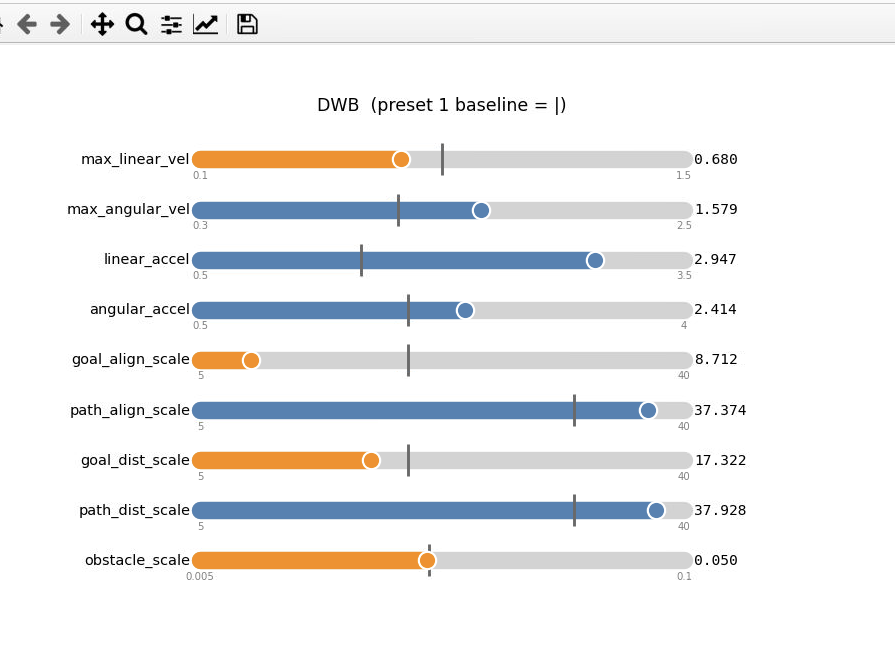
\includegraphics[width=\columnwidth]{./param_viz.png}
            \caption{Live parameter dial visualization during a training run. Each bar shows the current value relative to the preset baseline (vertical tick) and the full tunable range. Blue indicates the agent has pushed a parameter above baseline; orange indicates below.}
            \label{fig:param_viz}
        \end{figure}

        The tool proved useful for catching two failure modes that were not obvious from reward curves alone. In one case, the agent collapsed all parameters toward one extreme of their range and kept them there, which the dials made immediately apparent. In another case, the parameters were not changing at all between steps, which pointed to a bug in how actions were being applied rather than a training issue. Having a direct view of what the agent was actually doing to the planner at each step made these problems straightforward to diagnose.

        On top of the parameter visualizer, SB3 included wrappers for monitoring the training process in real time through TensorBoard. Since training would typically take several hours, this tool was absolutely necessary for stopping poor training iterations early due to bad sets of hyperparameter configurations (e.g. learning rates, batch sizes, etc.). In addition to allowing for stepping through training hyperparameter configurations more quickly; TensorBoard also allowed provided history for tracking trends across the different hyperparameter configuration and other design changes (see Figure~\ref{fig:tb_example} below).
        
        \begin{figure}[H]
            \centering
            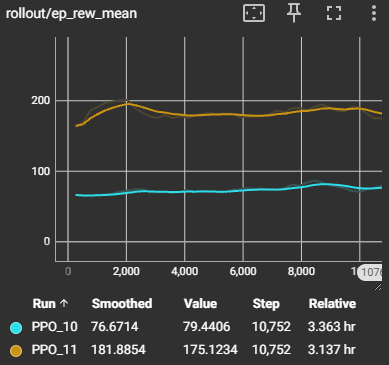
\includegraphics[scale=0.65]{./tensorboard_example.png}
            \caption{TensorBoard plot from PPO training before (blue--PPO\_10) and after (orange--PPO\_11) resolving a bug where episodes with aborted Nav2 path plans were rewarded with the same bonus as episodes which successfully reached the goal. Since drastically different results were given the same reward across episodes, the agent was confused about which actions were ``better'' and learning was ultimately stifled.}
            \label{fig:tb_example}
        \end{figure}

    \subsection{General Code Architecture}
    % Moved this after the RL architecture section for two reasons: 1) Huge chunk of our code is dedicated to RL and it doesn't make much sense to exclude it from this section 2) Including graphics here could minimize the amount of descriptive text needed in the "RL Architecture" section. If stuff starts getting wordy up there, we can just say "see Code Architecture section", or "see Figure __" and refer to figures here.
        \subsubsection{Planner control and Episode Runner}
        These two ROS2 nodes (planner\_controller.py and episode\_runner.py) work in concert and act as the backbone for the episodic training loop.
        The planner controller exposes three services: one to switch the active planner, one to apply a named preset, and one used by the RL bridge to
        push continuous parameter updates at each training step. When any of these are called, the node translates the logical parameter names into
        the ROS parameter names expected by Nav2 and forwards them directly to the controller server. It also keeps the velocity smoother's speed caps
        in sync and publishes a latched snapshot of the current parameter values for real-time diagnostics (see Figure~\ref{fig:planner_ctrl}).

        \begin{figure}[H]
        \centering
        \resizebox{\columnwidth}{!}{%
        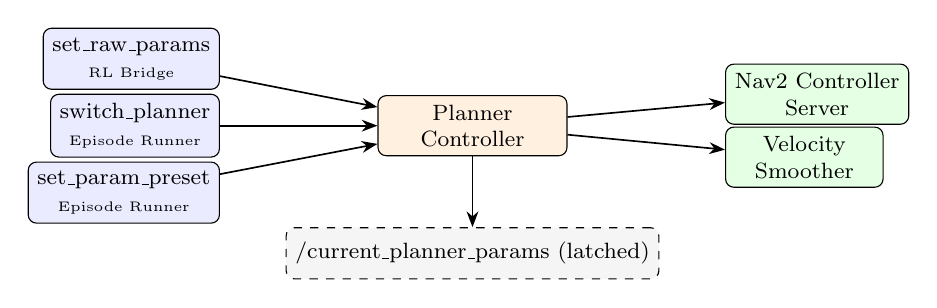
\begin{tikzpicture}[
          every node/.style={font=\footnotesize},
          box/.style={draw, rounded corners=3pt, minimum height=0.65cm, minimum width=2.0cm, align=center},
          srv/.style={box, fill=blue!8},
          nav/.style={box, fill=green!10},
          ctr/.style={box, fill=orange!12, minimum width=2.4cm},
          top/.style={box, dashed, fill=gray!8, minimum width=3.0cm},
          arr/.style={->, >=Stealth, semithick},
          lab/.style={font=\tiny, inner sep=1pt},
        ]
          \node[ctr] (ctrl) {Planner\\Controller};
          \node[srv, left=2.0cm of ctrl, yshift= 0.85cm] (raw)    {set\_raw\_params\\{\tiny RL Bridge}};
          \node[srv, left=2.0cm of ctrl]                 (switch) {switch\_planner\\{\tiny Episode Runner}};
          \node[srv, left=2.0cm of ctrl, yshift=-0.85cm] (preset) {set\_param\_preset\\{\tiny Episode Runner}};
          \node[nav, right=2.0cm of ctrl, yshift= 0.4cm] (nav2)   {Nav2 Controller\\Server};
          \node[nav, right=2.0cm of ctrl, yshift=-0.4cm] (smooth) {Velocity\\Smoother};
          \node[top, below=0.9cm of ctrl] (pub) {/current\_planner\_params (latched)};
          \draw[arr] (raw)    -- (ctrl);
          \draw[arr] (switch) -- (ctrl);
          \draw[arr] (preset) -- (ctrl);
          \draw[arr] (ctrl)   -- (nav2);
          \draw[arr] (ctrl)   -- (smooth);
          \draw[arr] (ctrl)   -- (pub);
        \end{tikzpicture}%
        }
        \caption{Planner Controller data flow. Services on the left accept requests from the RL bridge (continuous parameter updates) and the episode runner (planner/preset switching). Translated ROS parameters are pushed to the Nav2 controller server and velocity smoother; a latched snapshot is published for diagnostics.}
        \label{fig:planner_ctrl}
        \end{figure}

        The episode runner drives the training loop as a state machine. In benchmark mode it automatically cycles through planner and preset configurations,
        running each episode in sequence. In RL mode it waits after each episode until the training bridge calls \texttt{/start\_episode}, at which point
        it teleports the robot to the start pose, waits for the simulation to settle, resets the metrics tracker, and sends the navigation goal to Nav2.
        When the goal completes (or is cancelled on a collision), it collects the final episode metrics and publishes them for the RL bridge to consume
        as the episode's terminal signal. The full state machine is shown in Figure~\ref{fig:episode_runner}.

        \begin{figure}[H]
        \centering
        \resizebox{\columnwidth}{!}{%
        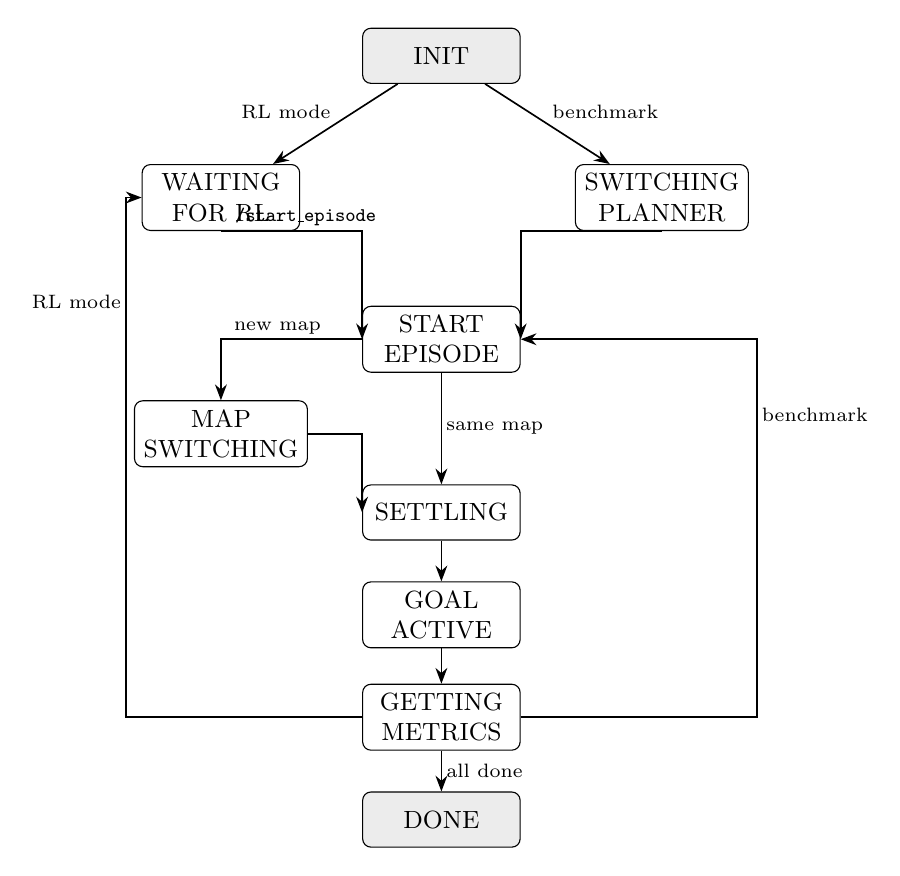
\begin{tikzpicture}[
          every node/.style={font=\small},
          state/.style={draw, rounded corners=3pt, minimum height=0.7cm, minimum width=2.0cm, align=center},
          arr/.style={->, >=Stealth, semithick},
          lab/.style={font=\scriptsize, inner sep=1.5pt},
        ]
          %% centre column — main sequence
          \node[state, fill=gray!15] (init)     at ( 0,   0.0) {INIT};
          \node[state]               (start)    at ( 0,  -3.6) {START\\EPISODE};
          \node[state]               (settling) at ( 0,  -5.8) {SETTLING};
          \node[state]               (goal)     at ( 0,  -7.1) {GOAL\\ACTIVE};
          \node[state]               (metrics)  at ( 0,  -8.4) {GETTING\\METRICS};
          \node[state, fill=gray!15] (done)     at ( 0,  -9.7) {DONE};
          %% left column
          \node[state]               (waiting)  at (-2.8, -1.8) {WAITING\\FOR RL};
          \node[state]               (map)      at (-2.8, -4.8) {MAP\\SWITCHING};
          %% right column
          \node[state]               (switching) at ( 2.8, -1.8) {SWITCHING\\PLANNER};

          %% INIT → mode branches
          \draw[arr] (init) -- node[lab,above left]{RL mode}    (waiting);
          \draw[arr] (init) -- node[lab,above right]{benchmark} (switching);

          %% side states → START (horizontal then down to west/east of start)
          \draw[arr] (waiting.south)   -| node[lab,above,pos=0.3]{\texttt{/start\_episode}} (start.west);
          \draw[arr] (switching.south) -| (start.east);

          %% START → branches
          \draw[arr] (start.west) -| node[lab,above,pos=0.3]{new map}  (map.north);
          \draw[arr] (start)       -- node[lab,right]{same map}         (settling);

          %% MAP → SETTLING
          \draw[arr] (map.east) -| (settling.west);

          %% main sequence
          \draw[arr] (settling) -- (goal);
          \draw[arr] (goal)     -- (metrics);
          \draw[arr] (metrics)  -- node[lab,right]{all done} (done);

          %% return loops — routed outside all nodes (x = ±4.0, beyond column edges ±3.8)
          \draw[arr] (metrics.west) -- ++(-3.0,0) |-
                     node[lab,left,pos=0.4]{RL mode}    (waiting.west);
          \draw[arr] (metrics.east) -- ++(3.0,0)  |-
                     node[lab,right,pos=0.4]{benchmark} (start.east);
        \end{tikzpicture}%
        }
        \caption{Episode runner state machine. In RL mode the node waits for \texttt{/start\_episode} service calls from the training bridge; in benchmark mode it advances automatically. After collecting end-of-episode metrics, it returns to \textsc{Waiting for RL} or advances to the next episode or planner configuration.}
        \label{fig:episode_runner}
        \end{figure}

\section{Experimentation}
    \subsection{Standard Path Planners}
    In order to determine the feasibility of constantly tuning planner parameters, the system was first tested by manually switching between two parameter sets for both MPPI and DWB. While DWB was able to handle the parameter changes without issue, MPPI struggled to keep moving when parameters were adjusted. This is due to the fact that MPPI relies on a sampling-based approach to generate its path, and when parameters are changed, the samples that were previously valid may no longer be valid, causing the planner to struggle to find a new path. Every time the parameter sets were changed, the robot would come to a stop, and then the planner would slowly resume planning motion. This is not ideal, and dramatically slows down the navigation process, defeating the purpose of this project. While it may be possible to mitigate this issue, the team decided to concentrate focus on the RL agent, and DWB was ultimately chosen to be the only planner that the RL agent would be trained on. DWB is a more traditional local planner that relies on a costmap-based approach, and it is able to handle parameter changes more gracefully than MPPI. This is because DWB generates its path based on the costmap, which is updated in real-time as the robot moves through the environment. As a result, when parameters are changed, DWB can quickly adapt to the new costmap and continue planning without significant disruption.
    
    \subsection{RL-Trained Planner: SAC Policy Agent}

        \subsubsection{SAC \& DWB Parameters Tuned}
        Four DWB parameters were selected for tuning to keep the action space small and learning tractable. Maximum linear velocity controls how fast the robot can move and has a direct effect on efficiency. Obstacle scale controls how aggressively DWB avoids obstacles when scoring candidate trajectories, governing the tradeoff between clearance and speed.

        The other two are meta-parameters: path weight and goal weight. Rather than tuning DWB's four critic scales independently, each meta-parameter scales a correlated pair together: path weight adjusts both path-following critics simultaneously, and goal weight adjusts both goal-seeking critics. This keeps the action space small without giving up meaningful control, since the two critics in each pair always push in the same direction anyway.

        \subsubsection{State and Action Space Design}
        The agent observes 12 values at each timestep: eight navigation state values and four values representing the agent's own currently active parameter settings. The navigation state includes three path-cost lookahead values sampled from the Nav2 costmap along the upcoming plan (covering roughly 1\,m, 3\,m, and 6\,m ahead), distance and heading error to the goal, linear velocity, angular velocity, and lateral deviation from the global plan. Raw LiDAR was excluded because the costmap lookahead already captures obstacle proximity in a form the planner directly acts on, and a smaller observation keeps learning more tractable. The agent's own smoothed parameter values are appended to the observation so the policy can see what settings are currently active in the planner.

        The action space is four continuous values, one per tunable parameter. The raw policy output is smoothed with an exponential moving average before being decoded into physical values and applied to Nav2, which prevents rapid swings from disrupting DWB mid-episode. Obstacle scale is decoded on a log scale since its useful range spans two orders of magnitude; the other three parameters are decoded linearly.

        \subsubsection{Reward Function Design and Tuning}
        The reward function was adjusted several times during training to address observed failure modes. The core signal is a progress reward for reducing distance to the goal each timestep, with smaller penalties on path deviation and angular velocity to encourage smooth, on-plan behavior. A graduated proximity penalty also activates when the planned path ahead enters an inflated obstacle region, growing as the path gets closer to the obstacle.

        Two terms were added during tuning. A direct collision penalty was added after observing that the proximity penalty alone was not a strong enough deterrent when the robot actually entered an obstacle cell. A slow-pace penalty was added to address cases where the agent learned to creep slowly through open areas, it only fires when the robot is far from the goal and well clear of obstacles, so it does not punish legitimate slowdowns near corners or as the robot approaches the goal.

        The original flat time penalty per timestep was replaced with a per-goal time-delta terminal reward that compares the agent's completion time against a pre-collected baseline time for that specific goal. This prevents longer routes from automatically producing larger penalties just because they take more time. Baseline times are gathered by running the fixed preset-1 configuration through all goal configurations before training begins. At episode end, a goal bonus of $+100$ is awarded for success and a failure penalty of $-50$ is applied otherwise. A collision also immediately ends the episode with the failure penalty rather than letting navigation continue, since recovery behavior from a collision tends to be erratic and unhelpful for training.

        % MOVING THIS FROM "RL ARCHITECTURE" SETION TO HERE FOR REFERENCE
        %The reward function was then built around five per-step terms (dense rewards) and two terminal terms (sparse rewards). Each term targets one of four relevant navigation quality criteria used for evaluation shown above. The primary signal is a progress reward proportional to the reduction in distance to the goal each timestep, which gives the agent a continuous incentive to move forward rather than waiting for a sparse goal signal at the end of the episode. Three penalty terms counterbalance this: a small penalty for deviating laterally from the global plan encourages the agent to stay on the intended path; a penalty on angular velocity discourages unnecessary spinning; and a graduated proximity penalty activates when the planned path ahead of the robot enters an inflated obstacle region on the costmap, increasing as the path gets closer to an obstacle. Unlike a binary collision flag, the graduated penalty provides a smooth signal that the agent can learn from without being destabilized by sudden large negative rewards. A flat time penalty is also applied every timestep regardless of other conditions, making overall navigation speed the dominant optimization pressure.

        %At the end of each episode, a goal bonus of $+100$ is awarded if the robot successfully reaches its destination, and a failure penalty of $-50$ is applied if the episode ends without reaching the goal. The larger bonus relative to the penalty is intentional, as it keeps the agent willing to attempt difficult routes rather than playing it safe and timing out.

    \subsection{RL-Trained Planner:PPO Policy Agent}
        \subsubsection{State and Action Space Design}
        The PPO agent observation space was designed to include information about ``what the robot sees'', ``where the robot thinks it is'', and ``where the robot thinks it's going''. For what the robot sees, the state vector includes space for a predefined set of $N$ downsampled lidar ranges and bearings. However, instead of downsampling the lidar measurements in fixed increments around the robot, the lidar rays were divided into $N$ segments; where the minimum range measurements and associated bearing angles are extracted from each individual segment. This ensures that lidar measurements associated with the closest features surrounding the robot make it into the state vector and are not ``missed'' or sampled out. The lidar segment design is illustrated in Figure \_ below.
        % placeholder for figure
        For where the robot thinks it is, the state vector included the error components for $x$, $y$, and yaw. The error components were selected over the global frame components for $x$, $y$, and yaw as an attempt to minimize the dimensionality of the state vector; because the agent would either require knowledge of the goal pose, or require knowledge of the map itself, in order to make sense of the global frame components. And from a function approximation perspective, it makes more sense intuitively to determine actions based on how far away the robot is from the goal over where the robot is located within a given map. This is especially true when the same global coordinates represent entirely different states across different maps. For where the robot thinks it's going, the state vector included the elements for the linear and angular velocity components of the robot. Since the Turtlebot that we're trying to control is a differential drive robot, the velocity components can be represented concisely by a single forward velocity term, $v$, and a single steering velocity term, $\omega$. All together, the state vector took the following form:
        \begin{gather*}
            s =
            \begin{bmatrix}
                r_{lidar\_0}  \\
                \theta_{lidar\_0} \\
                ... \\
                r_{lidar\_(N-1)} \\
                \theta_{lidar\_(N-1)} \\
                x_{err} \\
                y_{err} \\
                \theta_{err} \\
                v \\
                \omega \\
            \end{bmatrix}
        \end{gather*}
        where:
        \begin{itemize}
            \item $s$ is the state (observation) vector.
            \item $N$ is the number of lidar segments.
            \item $r_{lidar\_(N-1)}$ is the range of the shortest lidar return in segment $(N-1)$.
            \item $\theta_{lidar\_(N-1)}$ is the bearing (with respect to the robot) of the shortest lidar return in segment $(N-1)$.
            \item $x_{err}$ is the $x$-component of the error between the robot's current pose and the goal pose.
            \item $y_{err}$ is the $y$-component of the error between the robot's current pose and the goal pose.
            \item $\theta_{err}$ is the yaw-component of the error between the robot's current pose and the goal pose.
            \item $v$ is the linear (forward) velocity of the robot.
            \item $\omega$ is the rotational (steering) velocity of the robot.
        \end{itemize}
        While different configurations of the state vector were tested, the final state vector included lidar measurements from 18 segments ($N$=18); so the final state vector consisted of 41 elements.
        
        The PPO agent action space was specifically designed to configure how fast, and how smooth, the DWB planner should control the robot. Of course, this is all done indirectly by adjusting boundaries and constraints that the DWB planner can work within. For configuring how fast the robot is controlled, the action vector includes the DWB parameters that control both the maximum and minimum velocities (increasing the maximum velocity alone may not gaurantee that the robot will speed up without also increasing the minimum velocity). For controlling how smooth the robot is controlled, the action vector includes the DWB parameters which control both the goal seeking and path seeking weights. This indirectly influences the smoothness of the planner because it effectively tells DWB how closely it should follow the immediate waypoints within the global path versus ignoring the global path to a certain degree in favor of reaching the goal faster. All together, the action vector took the following form:
        \begin{gather*}
            a =
            \begin{bmatrix}
                v_{max} \\
                v_{min} \\
                GoalAlign.scale \\
                PathAlign.scale \\
                GoalDist.scale \\
                PathDist.scale \\
            \end{bmatrix}
        \end{gather*}
        where:
        \begin{itemize}
            \item $v_{max}$ is the DWB planner's ``max\_vel\_x" parameter (velocity ceiling).
            \item $v_{min}$ is the DWB planner's ``min\_speed\_xy" parameter (velocity floor).
            \item $GoalAlign.scale$ is the DWB planner's ``GoalAlign.scale" parameter (scores a trajectory based on how well aligned the trajectory is with the goal pose).
            \item $PathAlign.scale$ is the DWB planner's ``PathAlign.scale" parameter (scores a trajectory based on how well it is aligned to the path provided by the global planner).
            \item $GoalDist.scale$ is the DWB planner's ``GoalDist.scale" parameter (scores a trajectory based on how close the trajectory gets the robot to the goal pose).
            \item $PathDist.scale$ is the DWB planner's ``PathDist.scale" parameter (scores a trajectory based on how close the trajectory gets the robot to the trajectory of the global planner).
        \end{itemize}
        
        With the state and action spaces of the PPO agent defined, the feedback between the state and action mapping needed to be established. While the reward function plays a pivotal role in providing that feedback for the agent to learn from; additional control was needed to account for the asynchronous nature of ROS2, along with the Nav2 stack's sensitivity to large rapid changes. While the custom gymnasium environment was responsible for transmitting the action to Nav2, the underlying ROS2 environment had potential to propagate the action to the Nav2 stack and publish an observation for the next state simultaneously. Without intervention, there would be no way to gaurantee the operating assumption of RL environments where the next state is produced as a result of the recently applied action. And even though there is a way to gaurantee that the next state observation is published after the Nav2 action is applied (via ROS2 callback groups); the immediate next state observation that follows the applied Nav2 action isn't gauranteed to be ``useful'' information for the agent since the impact of the DWB planner adjustments may not have had time to be fully realized. So in order to provide enough time for the planner's current configuration to produce a meaningful next state, the PPO agent's custom gymnasium environment was programmed to wait for a pre-specified amount of time before accepting a newly published observation from ROS2. The final implementation of the PPO agent's environment ended up using a 1.0 second wait time, but this parameter could ultimately be treated as a hyperparameter and further optimized.  

        \subsubsection{Reward Function Design}
        The hybrid reward function for the PPO could be summarized as follows:
        \begin{gather*}
            R = r_{terminal} + r_{step} + r_{progress} + r_{smoothness} + r_{proximity}
        \end{gather*}
        where:
        \begin{gather*}
            r_{terminal} =
            \begin{dcases}
                R_{GOAL}    & \text{if goal reached} \\
                R_{COLL}    & \text{if collision occurred} \\
                0           & \text{otherwise} \\
            \end{dcases} \\
            \\
            r_{step} = R_{STEP} \\
            \\
            r_{progress} = R_{PROG}*(xy\_error_{last}-xy\_error_{current}) \\
            \\
            r_{smoothness} = R_{SMOOTH}*|\omega| \\
            \\
            r_{proximity} = R_{PROX}*(r_{threshold}-r_{min\_lidar}))
        \end{gather*}
        and the values of the final PPO agent implementation are contained in Table \ref{tab:ppo_values}.
        \begin{table}
            \centering
            \caption{PPO Agent Reward Function Constants}\label{tab:ppo_values}
            \begin{tabular}{|c|c|p{5cm}|}
                \hline
                \textbf{Parameter} & \textbf{Value} & \textbf{Description} \\
                \hline
                $R_{GOAL}$ & +100 & Sparse bonus for the robot successfully reaching the goal.\\
                \hline
                $R_{COLL}$ & -100 & Sparse penalty for when the robot experiences a collision.\\
                \hline
                $R_{STEP}$ & -0.01 & Dense penalty for steps through the environment meant to encourage faster paths toward the goal.\\
                \hline
                $R_{PROG}$ & +10.0 & Dense reward scale meant to encourage making progress towards the goal and discourage further distancing from the goal.\\
                \hline
                $R_{SMOOTH}$ & -0.01 & Dense reward scale meant to discourage unnecessary or jerky rotation.\\
                \hline
                $R_{PROX}$ & -1.0 & Dense reward scale meant to penalize the robot's proximity to environment features within the minimum range threshold, $r_{threshold}$. \\
                \hline
                $r_{threshold}$ & 1.0 & The minimum range threshold (in meters) which activates the proximity penalty. When lidar measurements fall below this threshold, the penalty is determined by scaling $R_{PROX}$ by the difference between the threshold and the minimum lidar range measurement.\\
                \hline
            \end{tabular}
        \end{table}

\section{Results}
% NOTE: In case somebody beats me to it, I dumped all my results into the ecw_tinkering branch in the following directory:
%   - ./rbe_capstone/rl_pipeline/rl_results.
% Was planning to add relevant training plots and summarize the .json into a table. For the training plots, my current plan is to include the full training plot (non clipped version) and use like a box or arrow to point to/notate where the checkpoint was taken from (10,000 steps).

% This should get into the comparisons, how much time was saved or not in navigation, if certian parameters had more effect, etc.
After conduction all -----NUMBER---- of experiments with both standard and RL-driven planners, it was made clear that -----BIG CONCLUSIVE RESULT-----

-----GRAPHIC OVERLAYS OF STANDARD / RL PERFORMANCE FOR CLEARANCE, ACCURACY, EFFICIENCY, AND SMOOTHNESS-----

Figures \ref{fig:view_tb} and \ref{fig:move_tb} below showcase the current state of the simulation environment as described above.
\begin{figure}[H]
    \centering
    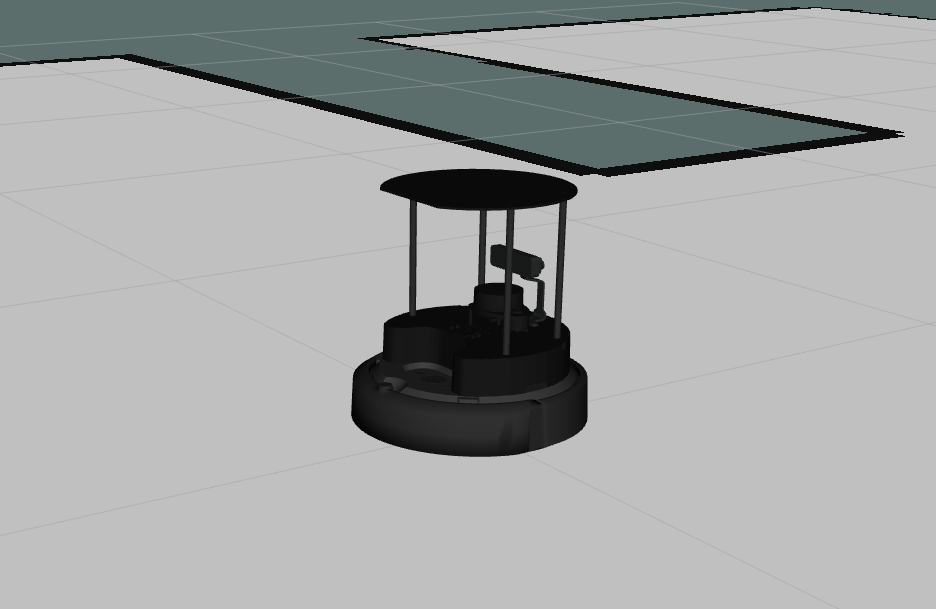
\includegraphics[scale=0.25]{./view_turtlebot.png}
    \caption{TurtleBot4 model loaded in RViz2 with a simple occupancy grid map environment for demonstration purposes.}
    \label{fig:view_tb}
\end{figure}

\begin{figure}[H]
    \centering
    \begin{subfigure}[b]{0.23\textwidth}
        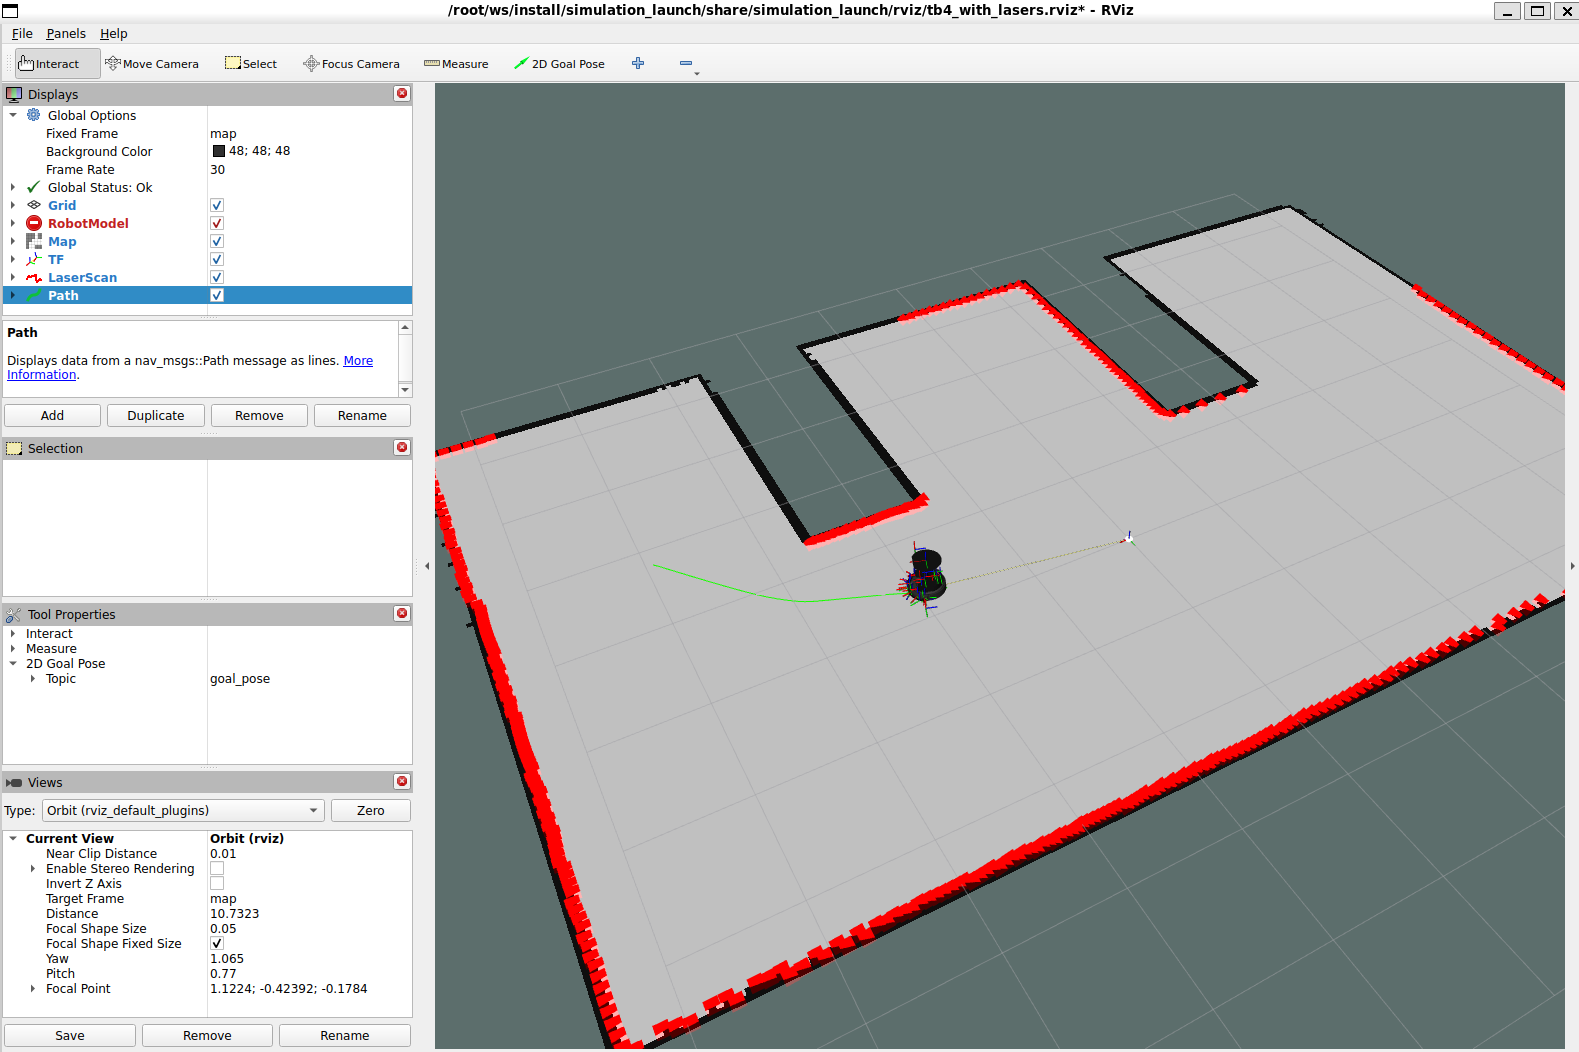
\includegraphics[scale=0.1]{./move_turtlebot_1.png}
        \subcaption{}
        \label{subfig:p1}
    \end{subfigure}
    \begin{subfigure}[b]{0.23\textwidth}
        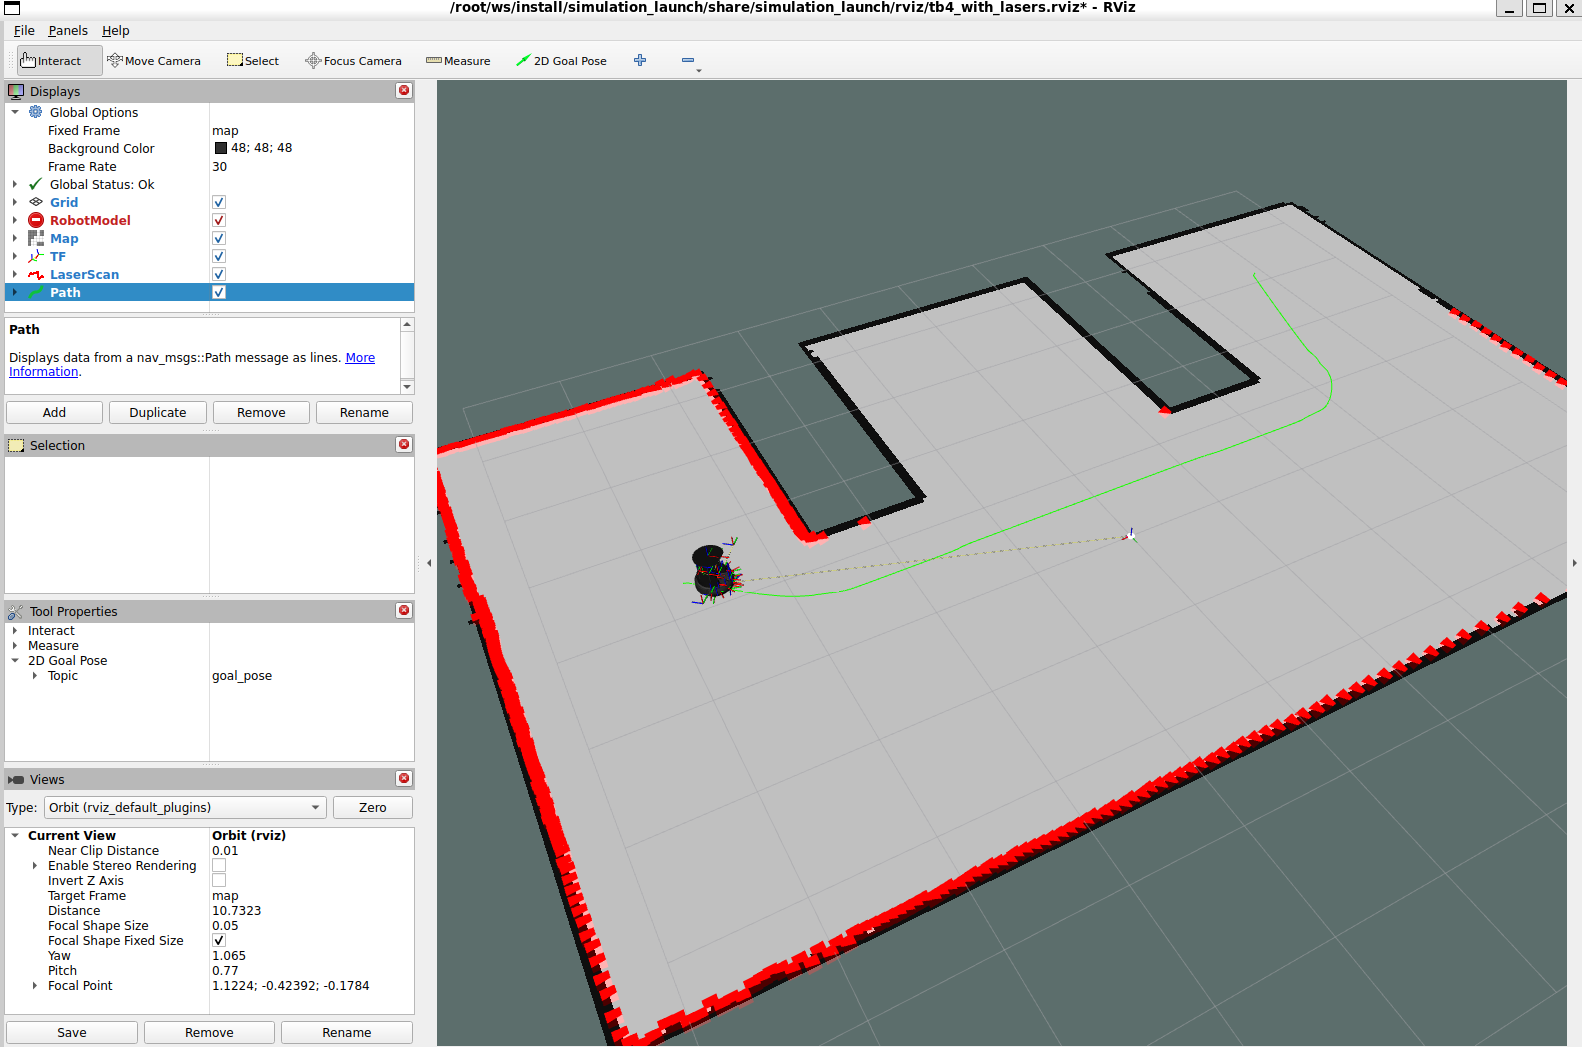
\includegraphics[scale=0.1]{./move_turtlebot_2.png}
        \subcaption{}
        \label{subfig:p2}
    \end{subfigure}
    \hfill
    \begin{subfigure}[b]{0.23\textwidth}
        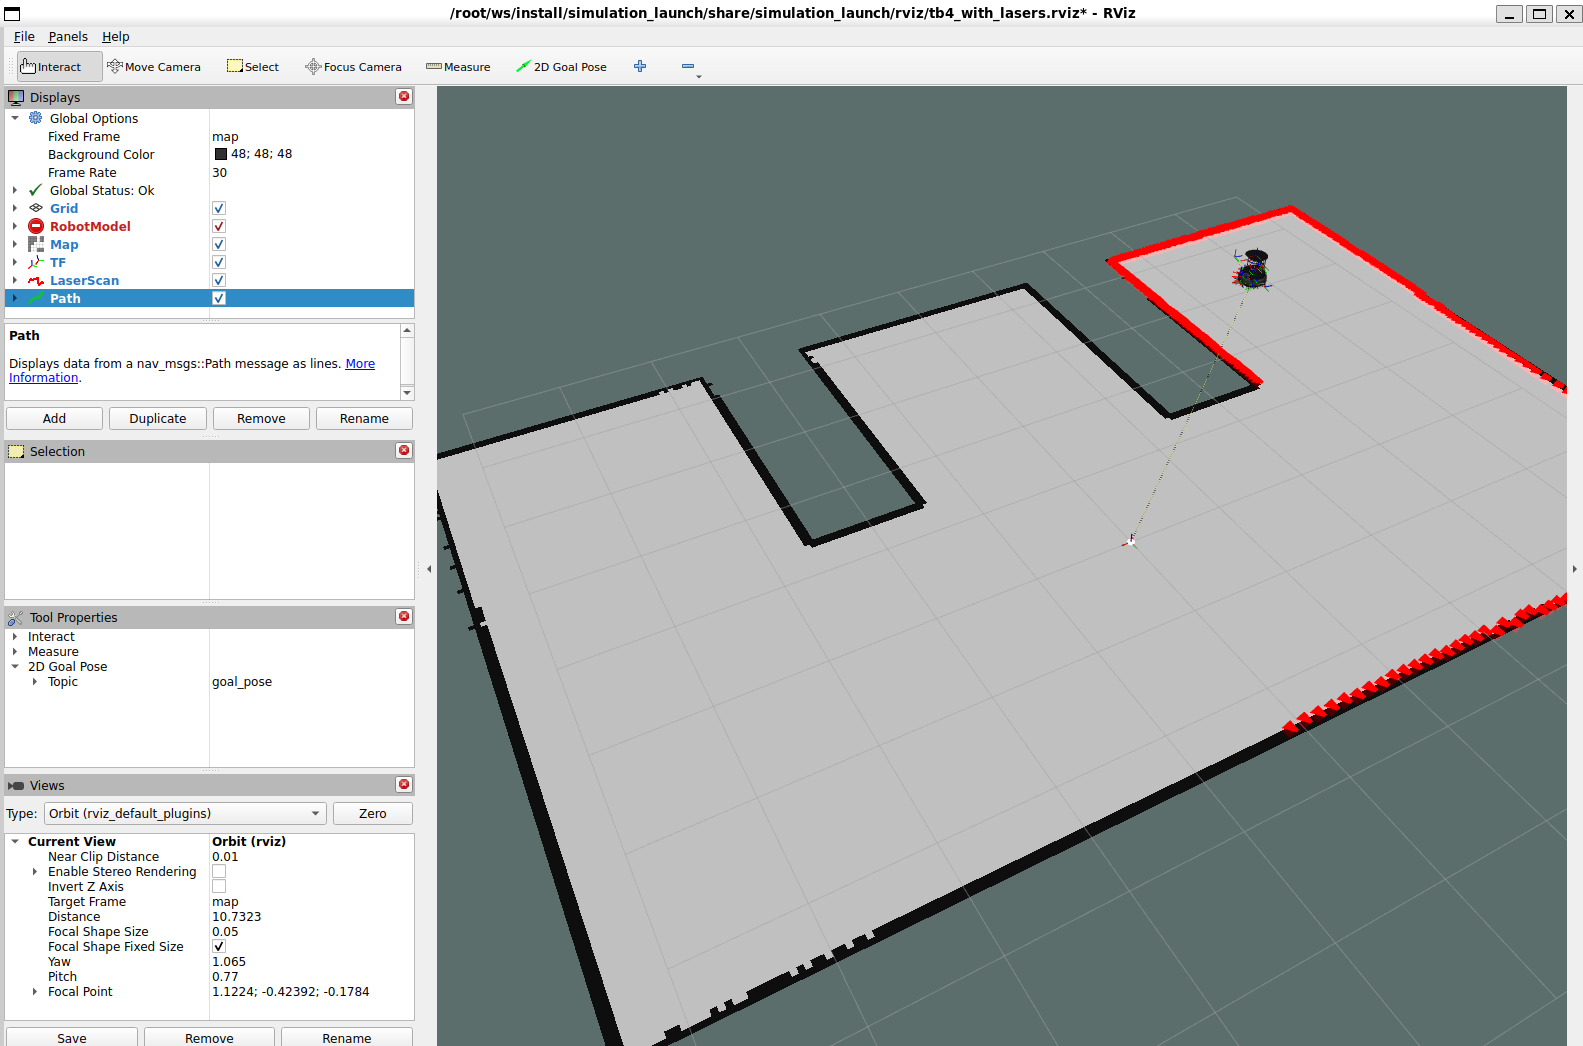
\includegraphics[scale=0.1]{./move_turtlebot_3.png}
        \subcaption{}
        \label{subfig:p3}
    \end{subfigure}
    \caption{TurtleBot4 model scanning and moving through the environment with goal poses set directly through RViz2. In \ref{subfig:p1}, the robot moves along the generated path (in green) from its initial pose to the first goal pose (in the upper left corner). Then in \ref{subfig:p2}, a new goal pose was commanded, resulting in a new path (to the upper right corner). Finally, in \ref{subfig:p3}, the robot reaches the final goal pose. All this navigation was done through manual control; and this sort of process will need to automated in order for the RL agent to be trained. Additionally, as the robot travels from \ref{subfig:p1} to \ref{subfig:p3}, it's clear from the LiDAR model scans (in red) that different parts of the environment become occluded. This is an important aspect of the environment that the RL agent will need to learn to account for when tuning the planner parameters.}
    \label{fig:move_tb}
\end{figure}

\section{Discussion}
    \subsection{Implications of Results}
    % What kind of benefits could be seen for the time saved, if any, is it statistically significant

    \subsection{Future Work}
    % Adding more path planners & the ability to switch between, trying a different RL agent policy (?) adding dynmaic obstacles, expanding to 3D / Gazebo

\newpage
\begin{thebibliography}{00}
\bibitem{b1} S. M. Elbouhy, A. Adamanov, P. M. Braun and H. Wilhelm Rose, "Comparative Analysis of Local Trajectory Planning Algorithms in ROS2," 2025 IEEE International Conference on Simulation, Modeling, and Programming for Autonomous Robots (SIMPAR), Palermo, Italy, 2025, pp. 1-6, doi: 10.1109/SIMPAR62925.2025.10979015.

\bibitem{b2} H. Li, W. Zhang, Z. Dong, J. Yang and J. Lu, "Local Path Planning Algorithm of Mobile Robot by Modified Optimized Parameters Method," 2021 IEEE 5th Advanced Information Technology, Electronic and Automation Control Conference (IAEAC), Chongqing, China, 2021, pp. 1014-1018, doi: 10.1109/IAEAC50856.2021.9391102.

\bibitem{b3} Y. Qu et al., "RL-Driven MPPI: Accelerating Online Control Laws Calculation With Offline Policy," in IEEE Transactions on Intelligent Vehicles, vol. 9, no. 2, pp. 3605-3616, Feb. 2024, doi: 10.1109/TIV.2023.3348134.

\bibitem{b4} L. Ting, H. B. Y. Ali and M. K. Chamran, "Accelerating Deep Reinforcement Learning for Mobile Robot Path Planning with Curriculum Learning and Reward Shaping," 2025 IEEE 9th International Conference on Software Engineering and Computer Systems (ICSECS), Pekan, Pahang, Malaysia, 2025, pp. 343-347, doi: 10.1109/ICSECS65227.2025.11279207.

\bibitem{b5} F. Pimentel and P. Aquino, “Performance Evaluation of ROS Local Trajectory Planning Algorithms to Social Navigation,” Oct. 2019, doi: \url{https://doi.org/10.1109/lars-sbr-wre48964.2019.00035}.

\bibitem{b6} Isira Naotunna and Theeraphong Wongratanaphisan, “Comparison of ROS Local Planners with Differential Drive Heavy Robotic System,” vol. 4, pp. 1-6, Dec. 2020, doi: \url{https://doi.org/10.1109/icamechs49982.2020.9310123}.

\bibitem{b7} C.-C. Wong, K.-D. Weng, and B.-Y. Yu, “Multi-Robot Navigation System Design Based on Proximal Policy Optimization Algorithm,” Information, vol. 15, no. 9, p. 518, Aug. 2024, doi: \url{https://doi.org/10.3390/info15090518}.

\bibitem{b8} F. Almeida, G. Le\~{a}o, and A. Sousa, “An Educational Kit for Simulated Robot Learning in ROS 2,” Robot 2023: Sixth Iberian Robotics Conference, vol. 2, pp. 513-525, doi: \url{https://doi.org/10.1007/978-3-031-59167-9_4}.

\bibitem{b9} A. Debnath, G. J. Stein, and J. Ko\v{s}eck\'{a}, "A Hybrid Approach to Indoor Social Navigation: Integrating Reactive Local Planning and Proactive Global Planning," \textit{2025 IEEE International Conference on Robotics and Automation (ICRA)}, Atlanta, USA, May 2025, pp. 10432--10438, doi: \url{https://doi.org/10.1109/ICRA55743.2025.11127475}.

\bibitem{b10} A. Rana and B. Kaveendran, "Deep Reinforcement Learning with PPO for Autonomous Mobile Robot Navigation Using ROS 2 Framework," \textit{International Journal for Research in Applied Science and Engineering Technology (IJRASET)}, vol. 13, no. VII, Jul. 2025, doi: \url{https://doi.org/10.22214/ijraset.2025.73330}.

\bibitem{b11} T. Haarnoja, A. Zhou, P. Abbeel, and S. Levine, “Soft Actor-Critic: Off-Policy Maximum Entropy Deep Reinforcement Learning with a Stochastic Actor,” arXiv (Cornell University), Jan. 2018, doi: \url{https://doi.org/10.48550/arxiv.1801.01290}.

\end{thebibliography}


\newpage
\onecolumn
\appendix
\section{Appendix}
  \subsection{Source Code}
    All the code for this project can be found in a Git repository here: [\url{https://github.com/SushiRaj99/rbe-capstone}] or seen below.
    \clearpage
    \newpage
\end{document}
